\documentclass[12pt,letterpaper]{article}
\usepackage[T1]{fontenc}
\usepackage[utf8]{inputenc}
\usepackage{helvet}
\renewcommand{\familydefault}{\sfdefault}
\usepackage[letterpaper,left=0.75in,right=0.75in,top=0.85in,bottom=0.85in,headheight=18pt,headsep=14pt,footskip=26pt]{geometry}
\usepackage{tikz}
\usepackage{pifont}
\usepackage{fancyhdr}
\definecolor{cred}{RGB}{214,39,40}
\definecolor{cblue}{RGB}{31,92,204}
\pagestyle{fancy}
\fancyhf{}
\renewcommand{\headrulewidth}{0pt}
\lhead{Week NN / Patterns you cannot avoid / Grades 2--3}
\lfoot{Bellingham Math Circle / Week NN / NN-23-v1}
\rfoot{\thepage}
\setlength{\parindent}{0pt}
\setlength{\parskip}{4pt}
\linespread{1.12}
\begin{document}
Color each square of a strip red or blue. The strip is good if no three equally spaced squares, such as 2, 5, 8 or 4, 5, 6, are all the same color.
\begin{center}
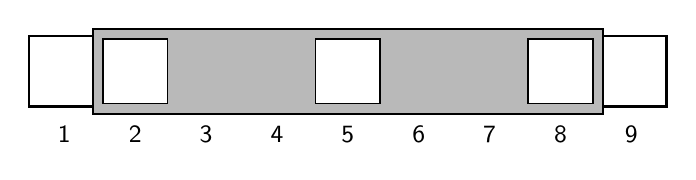
\begin{tikzpicture}
\draw[line width=0.9pt] (0.000,0.000) rectangle (0.900,0.900);
\node[font=\small, anchor=base] at (0.450,-0.450) {1};
\draw[line width=0.9pt] (0.900,0.000) rectangle (1.800,0.900);
\node[font=\small, anchor=base] at (1.350,-0.450) {2};
\draw[line width=0.9pt] (1.800,0.000) rectangle (2.700,0.900);
\node[font=\small, anchor=base] at (2.250,-0.450) {3};
\draw[line width=0.9pt] (2.700,0.000) rectangle (3.600,0.900);
\node[font=\small, anchor=base] at (3.150,-0.450) {4};
\draw[line width=0.9pt] (3.600,0.000) rectangle (4.500,0.900);
\node[font=\small, anchor=base] at (4.050,-0.450) {5};
\draw[line width=0.9pt] (4.500,0.000) rectangle (5.400,0.900);
\node[font=\small, anchor=base] at (4.950,-0.450) {6};
\draw[line width=0.9pt] (5.400,0.000) rectangle (6.300,0.900);
\node[font=\small, anchor=base] at (5.850,-0.450) {7};
\draw[line width=0.9pt] (6.300,0.000) rectangle (7.200,0.900);
\node[font=\small, anchor=base] at (6.750,-0.450) {8};
\draw[line width=0.9pt] (7.200,0.000) rectangle (8.100,0.900);
\node[font=\small, anchor=base] at (7.650,-0.450) {9};
\fill[gray!55, even odd rule] (0.810,-0.090) rectangle (7.290,0.990) (0.940,0.040) rectangle (1.760,0.860) (3.640,0.040) rectangle (4.460,0.860) (6.340,0.040) rectangle (7.160,0.860);
\draw[line width=0.8pt] (0.810,-0.090) rectangle (7.290,0.990);
\draw[line width=0.6pt] (0.940,0.040) rectangle (1.760,0.860);
\draw[line width=0.6pt] (3.640,0.040) rectangle (4.460,0.860);
\draw[line width=0.6pt] (6.340,0.040) rectangle (7.160,0.860);
\end{tikzpicture}
\end{center}\vspace{8pt}
\par\noindent\textbf{Problem 1:} What is the longest strip you can make good? Color your good strips.\par

\vspace{6pt}\begin{center}
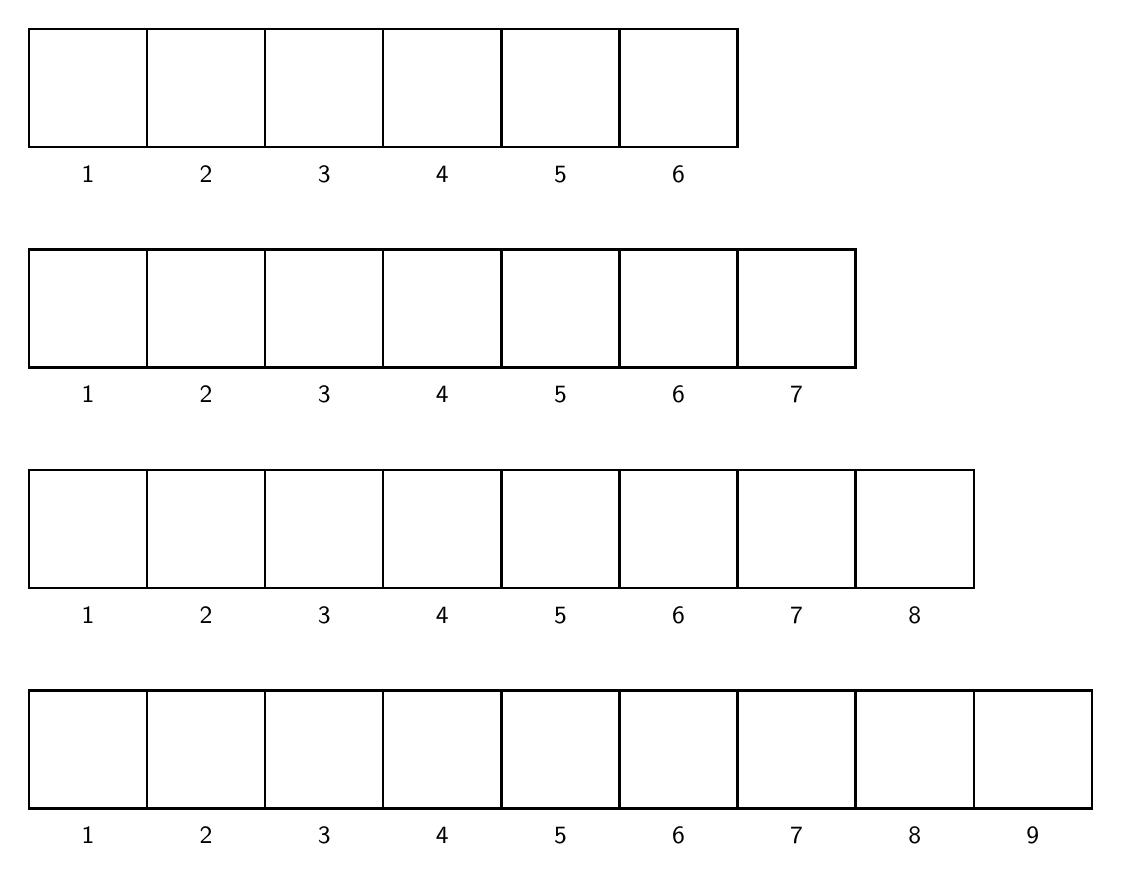
\begin{tikzpicture}
\draw[line width=0.9pt] (0.000,0.000) rectangle (1.500,1.500);
\node[font=\small, anchor=base] at (0.750,-0.450) {1};
\draw[line width=0.9pt] (1.500,0.000) rectangle (3.000,1.500);
\node[font=\small, anchor=base] at (2.250,-0.450) {2};
\draw[line width=0.9pt] (3.000,0.000) rectangle (4.500,1.500);
\node[font=\small, anchor=base] at (3.750,-0.450) {3};
\draw[line width=0.9pt] (4.500,0.000) rectangle (6.000,1.500);
\node[font=\small, anchor=base] at (5.250,-0.450) {4};
\draw[line width=0.9pt] (6.000,0.000) rectangle (7.500,1.500);
\node[font=\small, anchor=base] at (6.750,-0.450) {5};
\draw[line width=0.9pt] (7.500,0.000) rectangle (9.000,1.500);
\node[font=\small, anchor=base] at (8.250,-0.450) {6};
\draw[line width=0.9pt] (0.000,-2.800) rectangle (1.500,-1.300);
\node[font=\small, anchor=base] at (0.750,-3.250) {1};
\draw[line width=0.9pt] (1.500,-2.800) rectangle (3.000,-1.300);
\node[font=\small, anchor=base] at (2.250,-3.250) {2};
\draw[line width=0.9pt] (3.000,-2.800) rectangle (4.500,-1.300);
\node[font=\small, anchor=base] at (3.750,-3.250) {3};
\draw[line width=0.9pt] (4.500,-2.800) rectangle (6.000,-1.300);
\node[font=\small, anchor=base] at (5.250,-3.250) {4};
\draw[line width=0.9pt] (6.000,-2.800) rectangle (7.500,-1.300);
\node[font=\small, anchor=base] at (6.750,-3.250) {5};
\draw[line width=0.9pt] (7.500,-2.800) rectangle (9.000,-1.300);
\node[font=\small, anchor=base] at (8.250,-3.250) {6};
\draw[line width=0.9pt] (9.000,-2.800) rectangle (10.500,-1.300);
\node[font=\small, anchor=base] at (9.750,-3.250) {7};
\draw[line width=0.9pt] (0.000,-5.600) rectangle (1.500,-4.100);
\node[font=\small, anchor=base] at (0.750,-6.050) {1};
\draw[line width=0.9pt] (1.500,-5.600) rectangle (3.000,-4.100);
\node[font=\small, anchor=base] at (2.250,-6.050) {2};
\draw[line width=0.9pt] (3.000,-5.600) rectangle (4.500,-4.100);
\node[font=\small, anchor=base] at (3.750,-6.050) {3};
\draw[line width=0.9pt] (4.500,-5.600) rectangle (6.000,-4.100);
\node[font=\small, anchor=base] at (5.250,-6.050) {4};
\draw[line width=0.9pt] (6.000,-5.600) rectangle (7.500,-4.100);
\node[font=\small, anchor=base] at (6.750,-6.050) {5};
\draw[line width=0.9pt] (7.500,-5.600) rectangle (9.000,-4.100);
\node[font=\small, anchor=base] at (8.250,-6.050) {6};
\draw[line width=0.9pt] (9.000,-5.600) rectangle (10.500,-4.100);
\node[font=\small, anchor=base] at (9.750,-6.050) {7};
\draw[line width=0.9pt] (10.500,-5.600) rectangle (12.000,-4.100);
\node[font=\small, anchor=base] at (11.250,-6.050) {8};
\draw[line width=0.9pt] (0.000,-8.400) rectangle (1.500,-6.900);
\node[font=\small, anchor=base] at (0.750,-8.850) {1};
\draw[line width=0.9pt] (1.500,-8.400) rectangle (3.000,-6.900);
\node[font=\small, anchor=base] at (2.250,-8.850) {2};
\draw[line width=0.9pt] (3.000,-8.400) rectangle (4.500,-6.900);
\node[font=\small, anchor=base] at (3.750,-8.850) {3};
\draw[line width=0.9pt] (4.500,-8.400) rectangle (6.000,-6.900);
\node[font=\small, anchor=base] at (5.250,-8.850) {4};
\draw[line width=0.9pt] (6.000,-8.400) rectangle (7.500,-6.900);
\node[font=\small, anchor=base] at (6.750,-8.850) {5};
\draw[line width=0.9pt] (7.500,-8.400) rectangle (9.000,-6.900);
\node[font=\small, anchor=base] at (8.250,-8.850) {6};
\draw[line width=0.9pt] (9.000,-8.400) rectangle (10.500,-6.900);
\node[font=\small, anchor=base] at (9.750,-8.850) {7};
\draw[line width=0.9pt] (10.500,-8.400) rectangle (12.000,-6.900);
\node[font=\small, anchor=base] at (11.250,-8.850) {8};
\draw[line width=0.9pt] (12.000,-8.400) rectangle (13.500,-6.900);
\node[font=\small, anchor=base] at (12.750,-8.850) {9};
\end{tikzpicture}
\end{center}
\newpage
\par\noindent\textbf{Problem 2:} Find every good way to color a strip of 8 squares.\par

\vspace{6pt}\begin{center}
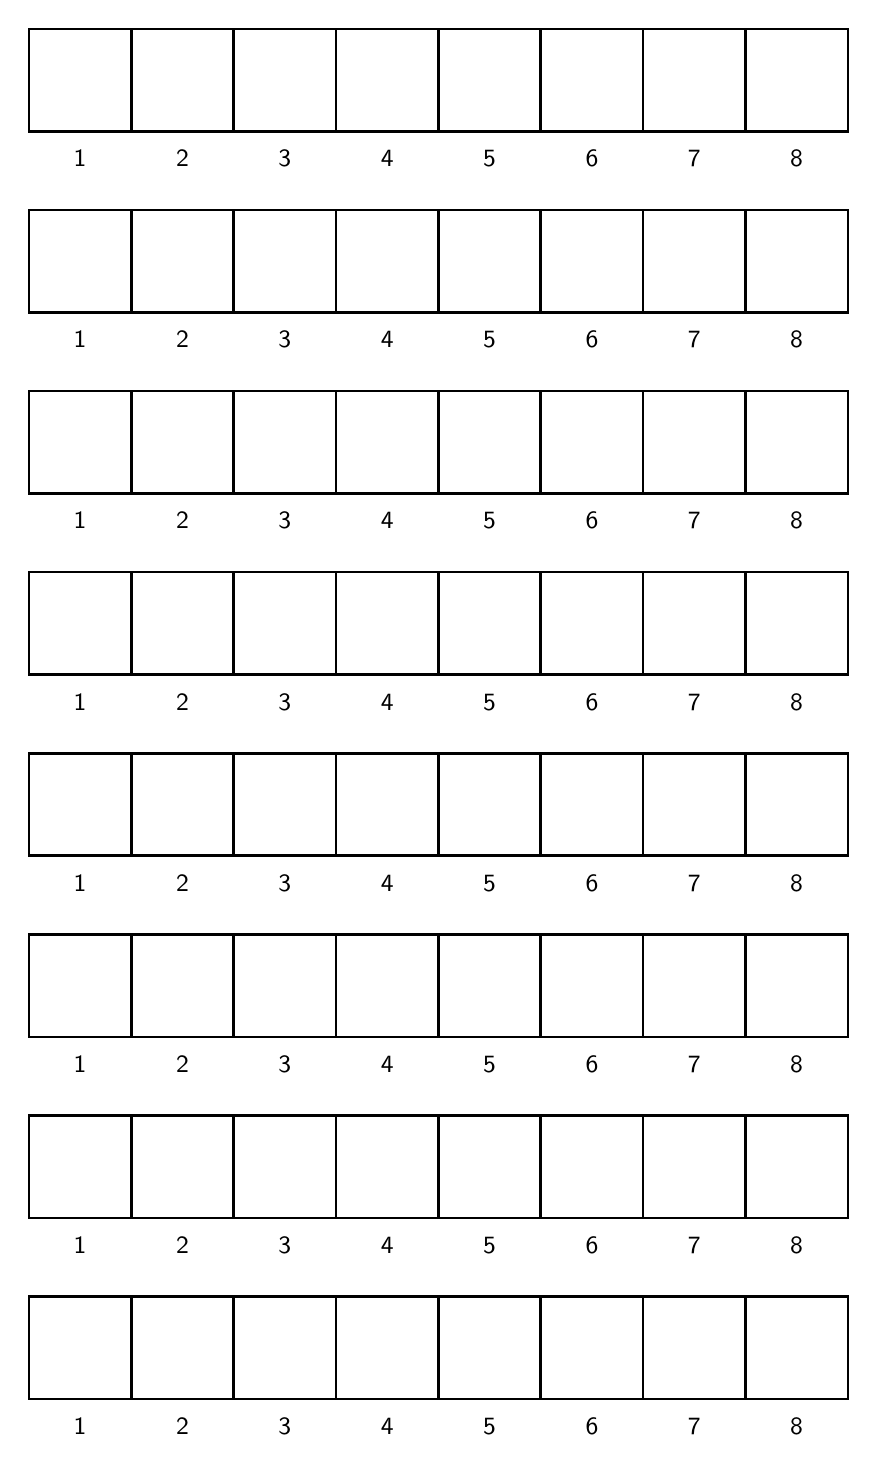
\begin{tikzpicture}
\draw[line width=0.9pt] (0.000,0.000) rectangle (1.300,1.300);
\node[font=\small, anchor=base] at (0.650,-0.450) {1};
\draw[line width=0.9pt] (1.300,0.000) rectangle (2.600,1.300);
\node[font=\small, anchor=base] at (1.950,-0.450) {2};
\draw[line width=0.9pt] (2.600,0.000) rectangle (3.900,1.300);
\node[font=\small, anchor=base] at (3.250,-0.450) {3};
\draw[line width=0.9pt] (3.900,0.000) rectangle (5.200,1.300);
\node[font=\small, anchor=base] at (4.550,-0.450) {4};
\draw[line width=0.9pt] (5.200,0.000) rectangle (6.500,1.300);
\node[font=\small, anchor=base] at (5.850,-0.450) {5};
\draw[line width=0.9pt] (6.500,0.000) rectangle (7.800,1.300);
\node[font=\small, anchor=base] at (7.150,-0.450) {6};
\draw[line width=0.9pt] (7.800,0.000) rectangle (9.100,1.300);
\node[font=\small, anchor=base] at (8.450,-0.450) {7};
\draw[line width=0.9pt] (9.100,0.000) rectangle (10.400,1.300);
\node[font=\small, anchor=base] at (9.750,-0.450) {8};
\draw[line width=0.9pt] (0.000,-2.300) rectangle (1.300,-1.000);
\node[font=\small, anchor=base] at (0.650,-2.750) {1};
\draw[line width=0.9pt] (1.300,-2.300) rectangle (2.600,-1.000);
\node[font=\small, anchor=base] at (1.950,-2.750) {2};
\draw[line width=0.9pt] (2.600,-2.300) rectangle (3.900,-1.000);
\node[font=\small, anchor=base] at (3.250,-2.750) {3};
\draw[line width=0.9pt] (3.900,-2.300) rectangle (5.200,-1.000);
\node[font=\small, anchor=base] at (4.550,-2.750) {4};
\draw[line width=0.9pt] (5.200,-2.300) rectangle (6.500,-1.000);
\node[font=\small, anchor=base] at (5.850,-2.750) {5};
\draw[line width=0.9pt] (6.500,-2.300) rectangle (7.800,-1.000);
\node[font=\small, anchor=base] at (7.150,-2.750) {6};
\draw[line width=0.9pt] (7.800,-2.300) rectangle (9.100,-1.000);
\node[font=\small, anchor=base] at (8.450,-2.750) {7};
\draw[line width=0.9pt] (9.100,-2.300) rectangle (10.400,-1.000);
\node[font=\small, anchor=base] at (9.750,-2.750) {8};
\draw[line width=0.9pt] (0.000,-4.600) rectangle (1.300,-3.300);
\node[font=\small, anchor=base] at (0.650,-5.050) {1};
\draw[line width=0.9pt] (1.300,-4.600) rectangle (2.600,-3.300);
\node[font=\small, anchor=base] at (1.950,-5.050) {2};
\draw[line width=0.9pt] (2.600,-4.600) rectangle (3.900,-3.300);
\node[font=\small, anchor=base] at (3.250,-5.050) {3};
\draw[line width=0.9pt] (3.900,-4.600) rectangle (5.200,-3.300);
\node[font=\small, anchor=base] at (4.550,-5.050) {4};
\draw[line width=0.9pt] (5.200,-4.600) rectangle (6.500,-3.300);
\node[font=\small, anchor=base] at (5.850,-5.050) {5};
\draw[line width=0.9pt] (6.500,-4.600) rectangle (7.800,-3.300);
\node[font=\small, anchor=base] at (7.150,-5.050) {6};
\draw[line width=0.9pt] (7.800,-4.600) rectangle (9.100,-3.300);
\node[font=\small, anchor=base] at (8.450,-5.050) {7};
\draw[line width=0.9pt] (9.100,-4.600) rectangle (10.400,-3.300);
\node[font=\small, anchor=base] at (9.750,-5.050) {8};
\draw[line width=0.9pt] (0.000,-6.900) rectangle (1.300,-5.600);
\node[font=\small, anchor=base] at (0.650,-7.350) {1};
\draw[line width=0.9pt] (1.300,-6.900) rectangle (2.600,-5.600);
\node[font=\small, anchor=base] at (1.950,-7.350) {2};
\draw[line width=0.9pt] (2.600,-6.900) rectangle (3.900,-5.600);
\node[font=\small, anchor=base] at (3.250,-7.350) {3};
\draw[line width=0.9pt] (3.900,-6.900) rectangle (5.200,-5.600);
\node[font=\small, anchor=base] at (4.550,-7.350) {4};
\draw[line width=0.9pt] (5.200,-6.900) rectangle (6.500,-5.600);
\node[font=\small, anchor=base] at (5.850,-7.350) {5};
\draw[line width=0.9pt] (6.500,-6.900) rectangle (7.800,-5.600);
\node[font=\small, anchor=base] at (7.150,-7.350) {6};
\draw[line width=0.9pt] (7.800,-6.900) rectangle (9.100,-5.600);
\node[font=\small, anchor=base] at (8.450,-7.350) {7};
\draw[line width=0.9pt] (9.100,-6.900) rectangle (10.400,-5.600);
\node[font=\small, anchor=base] at (9.750,-7.350) {8};
\draw[line width=0.9pt] (0.000,-9.200) rectangle (1.300,-7.900);
\node[font=\small, anchor=base] at (0.650,-9.650) {1};
\draw[line width=0.9pt] (1.300,-9.200) rectangle (2.600,-7.900);
\node[font=\small, anchor=base] at (1.950,-9.650) {2};
\draw[line width=0.9pt] (2.600,-9.200) rectangle (3.900,-7.900);
\node[font=\small, anchor=base] at (3.250,-9.650) {3};
\draw[line width=0.9pt] (3.900,-9.200) rectangle (5.200,-7.900);
\node[font=\small, anchor=base] at (4.550,-9.650) {4};
\draw[line width=0.9pt] (5.200,-9.200) rectangle (6.500,-7.900);
\node[font=\small, anchor=base] at (5.850,-9.650) {5};
\draw[line width=0.9pt] (6.500,-9.200) rectangle (7.800,-7.900);
\node[font=\small, anchor=base] at (7.150,-9.650) {6};
\draw[line width=0.9pt] (7.800,-9.200) rectangle (9.100,-7.900);
\node[font=\small, anchor=base] at (8.450,-9.650) {7};
\draw[line width=0.9pt] (9.100,-9.200) rectangle (10.400,-7.900);
\node[font=\small, anchor=base] at (9.750,-9.650) {8};
\draw[line width=0.9pt] (0.000,-11.500) rectangle (1.300,-10.200);
\node[font=\small, anchor=base] at (0.650,-11.950) {1};
\draw[line width=0.9pt] (1.300,-11.500) rectangle (2.600,-10.200);
\node[font=\small, anchor=base] at (1.950,-11.950) {2};
\draw[line width=0.9pt] (2.600,-11.500) rectangle (3.900,-10.200);
\node[font=\small, anchor=base] at (3.250,-11.950) {3};
\draw[line width=0.9pt] (3.900,-11.500) rectangle (5.200,-10.200);
\node[font=\small, anchor=base] at (4.550,-11.950) {4};
\draw[line width=0.9pt] (5.200,-11.500) rectangle (6.500,-10.200);
\node[font=\small, anchor=base] at (5.850,-11.950) {5};
\draw[line width=0.9pt] (6.500,-11.500) rectangle (7.800,-10.200);
\node[font=\small, anchor=base] at (7.150,-11.950) {6};
\draw[line width=0.9pt] (7.800,-11.500) rectangle (9.100,-10.200);
\node[font=\small, anchor=base] at (8.450,-11.950) {7};
\draw[line width=0.9pt] (9.100,-11.500) rectangle (10.400,-10.200);
\node[font=\small, anchor=base] at (9.750,-11.950) {8};
\draw[line width=0.9pt] (0.000,-13.800) rectangle (1.300,-12.500);
\node[font=\small, anchor=base] at (0.650,-14.250) {1};
\draw[line width=0.9pt] (1.300,-13.800) rectangle (2.600,-12.500);
\node[font=\small, anchor=base] at (1.950,-14.250) {2};
\draw[line width=0.9pt] (2.600,-13.800) rectangle (3.900,-12.500);
\node[font=\small, anchor=base] at (3.250,-14.250) {3};
\draw[line width=0.9pt] (3.900,-13.800) rectangle (5.200,-12.500);
\node[font=\small, anchor=base] at (4.550,-14.250) {4};
\draw[line width=0.9pt] (5.200,-13.800) rectangle (6.500,-12.500);
\node[font=\small, anchor=base] at (5.850,-14.250) {5};
\draw[line width=0.9pt] (6.500,-13.800) rectangle (7.800,-12.500);
\node[font=\small, anchor=base] at (7.150,-14.250) {6};
\draw[line width=0.9pt] (7.800,-13.800) rectangle (9.100,-12.500);
\node[font=\small, anchor=base] at (8.450,-14.250) {7};
\draw[line width=0.9pt] (9.100,-13.800) rectangle (10.400,-12.500);
\node[font=\small, anchor=base] at (9.750,-14.250) {8};
\draw[line width=0.9pt] (0.000,-16.100) rectangle (1.300,-14.800);
\node[font=\small, anchor=base] at (0.650,-16.550) {1};
\draw[line width=0.9pt] (1.300,-16.100) rectangle (2.600,-14.800);
\node[font=\small, anchor=base] at (1.950,-16.550) {2};
\draw[line width=0.9pt] (2.600,-16.100) rectangle (3.900,-14.800);
\node[font=\small, anchor=base] at (3.250,-16.550) {3};
\draw[line width=0.9pt] (3.900,-16.100) rectangle (5.200,-14.800);
\node[font=\small, anchor=base] at (4.550,-16.550) {4};
\draw[line width=0.9pt] (5.200,-16.100) rectangle (6.500,-14.800);
\node[font=\small, anchor=base] at (5.850,-16.550) {5};
\draw[line width=0.9pt] (6.500,-16.100) rectangle (7.800,-14.800);
\node[font=\small, anchor=base] at (7.150,-16.550) {6};
\draw[line width=0.9pt] (7.800,-16.100) rectangle (9.100,-14.800);
\node[font=\small, anchor=base] at (8.450,-16.550) {7};
\draw[line width=0.9pt] (9.100,-16.100) rectangle (10.400,-14.800);
\node[font=\small, anchor=base] at (9.750,-16.550) {8};
\end{tikzpicture}
\end{center}
\newpage
\par\noindent\textbf{Problem 3:} Can a strip of 9 squares be good? Explain how you know.\par

\vspace{6pt}\begin{center}
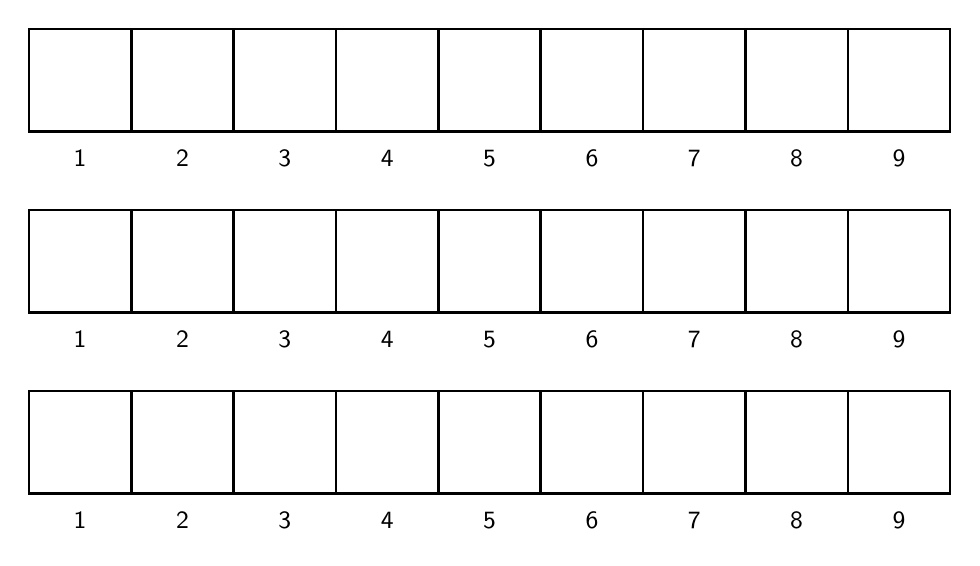
\begin{tikzpicture}
\draw[line width=0.9pt] (0.000,0.000) rectangle (1.300,1.300);
\node[font=\small, anchor=base] at (0.650,-0.450) {1};
\draw[line width=0.9pt] (1.300,0.000) rectangle (2.600,1.300);
\node[font=\small, anchor=base] at (1.950,-0.450) {2};
\draw[line width=0.9pt] (2.600,0.000) rectangle (3.900,1.300);
\node[font=\small, anchor=base] at (3.250,-0.450) {3};
\draw[line width=0.9pt] (3.900,0.000) rectangle (5.200,1.300);
\node[font=\small, anchor=base] at (4.550,-0.450) {4};
\draw[line width=0.9pt] (5.200,0.000) rectangle (6.500,1.300);
\node[font=\small, anchor=base] at (5.850,-0.450) {5};
\draw[line width=0.9pt] (6.500,0.000) rectangle (7.800,1.300);
\node[font=\small, anchor=base] at (7.150,-0.450) {6};
\draw[line width=0.9pt] (7.800,0.000) rectangle (9.100,1.300);
\node[font=\small, anchor=base] at (8.450,-0.450) {7};
\draw[line width=0.9pt] (9.100,0.000) rectangle (10.400,1.300);
\node[font=\small, anchor=base] at (9.750,-0.450) {8};
\draw[line width=0.9pt] (10.400,0.000) rectangle (11.700,1.300);
\node[font=\small, anchor=base] at (11.050,-0.450) {9};
\draw[line width=0.9pt] (0.000,-2.300) rectangle (1.300,-1.000);
\node[font=\small, anchor=base] at (0.650,-2.750) {1};
\draw[line width=0.9pt] (1.300,-2.300) rectangle (2.600,-1.000);
\node[font=\small, anchor=base] at (1.950,-2.750) {2};
\draw[line width=0.9pt] (2.600,-2.300) rectangle (3.900,-1.000);
\node[font=\small, anchor=base] at (3.250,-2.750) {3};
\draw[line width=0.9pt] (3.900,-2.300) rectangle (5.200,-1.000);
\node[font=\small, anchor=base] at (4.550,-2.750) {4};
\draw[line width=0.9pt] (5.200,-2.300) rectangle (6.500,-1.000);
\node[font=\small, anchor=base] at (5.850,-2.750) {5};
\draw[line width=0.9pt] (6.500,-2.300) rectangle (7.800,-1.000);
\node[font=\small, anchor=base] at (7.150,-2.750) {6};
\draw[line width=0.9pt] (7.800,-2.300) rectangle (9.100,-1.000);
\node[font=\small, anchor=base] at (8.450,-2.750) {7};
\draw[line width=0.9pt] (9.100,-2.300) rectangle (10.400,-1.000);
\node[font=\small, anchor=base] at (9.750,-2.750) {8};
\draw[line width=0.9pt] (10.400,-2.300) rectangle (11.700,-1.000);
\node[font=\small, anchor=base] at (11.050,-2.750) {9};
\draw[line width=0.9pt] (0.000,-4.600) rectangle (1.300,-3.300);
\node[font=\small, anchor=base] at (0.650,-5.050) {1};
\draw[line width=0.9pt] (1.300,-4.600) rectangle (2.600,-3.300);
\node[font=\small, anchor=base] at (1.950,-5.050) {2};
\draw[line width=0.9pt] (2.600,-4.600) rectangle (3.900,-3.300);
\node[font=\small, anchor=base] at (3.250,-5.050) {3};
\draw[line width=0.9pt] (3.900,-4.600) rectangle (5.200,-3.300);
\node[font=\small, anchor=base] at (4.550,-5.050) {4};
\draw[line width=0.9pt] (5.200,-4.600) rectangle (6.500,-3.300);
\node[font=\small, anchor=base] at (5.850,-5.050) {5};
\draw[line width=0.9pt] (6.500,-4.600) rectangle (7.800,-3.300);
\node[font=\small, anchor=base] at (7.150,-5.050) {6};
\draw[line width=0.9pt] (7.800,-4.600) rectangle (9.100,-3.300);
\node[font=\small, anchor=base] at (8.450,-5.050) {7};
\draw[line width=0.9pt] (9.100,-4.600) rectangle (10.400,-3.300);
\node[font=\small, anchor=base] at (9.750,-5.050) {8};
\draw[line width=0.9pt] (10.400,-4.600) rectangle (11.700,-3.300);
\node[font=\small, anchor=base] at (11.050,-5.050) {9};
\end{tikzpicture}
\end{center}
\newpage
\par\noindent\textbf{Problem 4:} Put a red or a blue counter on each of the cards 1, 2, 3 and 4. If two of the numbers add up to another one, like 1 + 3 = 4, those three numbers must not all be the same color. A number can be added to itself: 2 + 2 = 4, so 2 and 4 cannot be the same color. Find every way to color the cards.\par

\vspace{6pt}\begin{center}
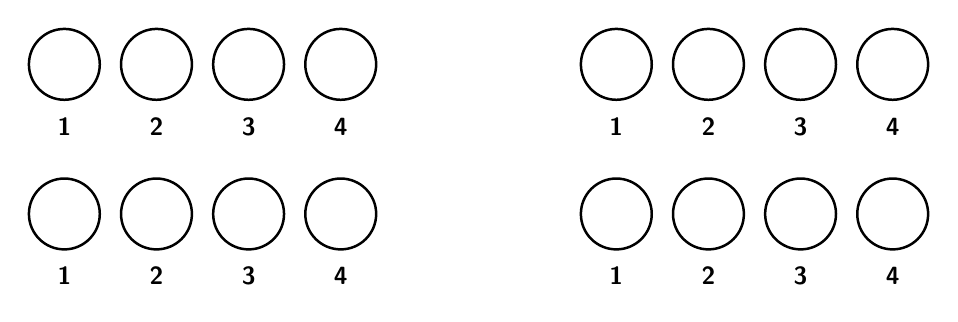
\begin{tikzpicture}
\draw[line width=0.9pt] (0.450,0.450) circle (0.450);
\node[font=\small\bfseries, anchor=base] at (0.450,-0.450) {1};
\draw[line width=0.9pt] (1.620,0.450) circle (0.450);
\node[font=\small\bfseries, anchor=base] at (1.620,-0.450) {2};
\draw[line width=0.9pt] (2.790,0.450) circle (0.450);
\node[font=\small\bfseries, anchor=base] at (2.790,-0.450) {3};
\draw[line width=0.9pt] (3.960,0.450) circle (0.450);
\node[font=\small\bfseries, anchor=base] at (3.960,-0.450) {4};
\draw[line width=0.9pt] (7.460,0.450) circle (0.450);
\node[font=\small\bfseries, anchor=base] at (7.460,-0.450) {1};
\draw[line width=0.9pt] (8.630,0.450) circle (0.450);
\node[font=\small\bfseries, anchor=base] at (8.630,-0.450) {2};
\draw[line width=0.9pt] (9.800,0.450) circle (0.450);
\node[font=\small\bfseries, anchor=base] at (9.800,-0.450) {3};
\draw[line width=0.9pt] (10.970,0.450) circle (0.450);
\node[font=\small\bfseries, anchor=base] at (10.970,-0.450) {4};
\draw[line width=0.9pt] (0.450,-1.450) circle (0.450);
\node[font=\small\bfseries, anchor=base] at (0.450,-2.350) {1};
\draw[line width=0.9pt] (1.620,-1.450) circle (0.450);
\node[font=\small\bfseries, anchor=base] at (1.620,-2.350) {2};
\draw[line width=0.9pt] (2.790,-1.450) circle (0.450);
\node[font=\small\bfseries, anchor=base] at (2.790,-2.350) {3};
\draw[line width=0.9pt] (3.960,-1.450) circle (0.450);
\node[font=\small\bfseries, anchor=base] at (3.960,-2.350) {4};
\draw[line width=0.9pt] (7.460,-1.450) circle (0.450);
\node[font=\small\bfseries, anchor=base] at (7.460,-2.350) {1};
\draw[line width=0.9pt] (8.630,-1.450) circle (0.450);
\node[font=\small\bfseries, anchor=base] at (8.630,-2.350) {2};
\draw[line width=0.9pt] (9.800,-1.450) circle (0.450);
\node[font=\small\bfseries, anchor=base] at (9.800,-2.350) {3};
\draw[line width=0.9pt] (10.970,-1.450) circle (0.450);
\node[font=\small\bfseries, anchor=base] at (10.970,-2.350) {4};
\end{tikzpicture}
\end{center}
\vspace{2.0cm}
\par\noindent\textbf{Problem 5:} Can the cards 1, 2, 3, 4 and 5 be colored by the same rule? Explain how you know.\par

\vspace{6pt}\begin{center}
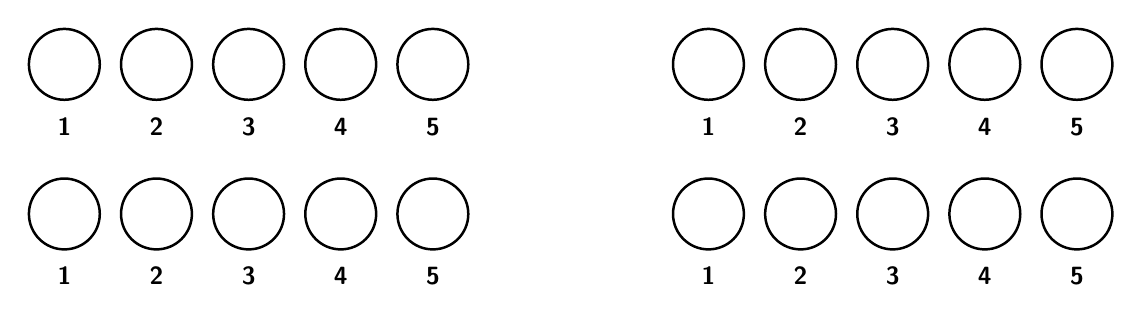
\begin{tikzpicture}
\draw[line width=0.9pt] (0.450,0.450) circle (0.450);
\node[font=\small\bfseries, anchor=base] at (0.450,-0.450) {1};
\draw[line width=0.9pt] (1.620,0.450) circle (0.450);
\node[font=\small\bfseries, anchor=base] at (1.620,-0.450) {2};
\draw[line width=0.9pt] (2.790,0.450) circle (0.450);
\node[font=\small\bfseries, anchor=base] at (2.790,-0.450) {3};
\draw[line width=0.9pt] (3.960,0.450) circle (0.450);
\node[font=\small\bfseries, anchor=base] at (3.960,-0.450) {4};
\draw[line width=0.9pt] (5.130,0.450) circle (0.450);
\node[font=\small\bfseries, anchor=base] at (5.130,-0.450) {5};
\draw[line width=0.9pt] (8.630,0.450) circle (0.450);
\node[font=\small\bfseries, anchor=base] at (8.630,-0.450) {1};
\draw[line width=0.9pt] (9.800,0.450) circle (0.450);
\node[font=\small\bfseries, anchor=base] at (9.800,-0.450) {2};
\draw[line width=0.9pt] (10.970,0.450) circle (0.450);
\node[font=\small\bfseries, anchor=base] at (10.970,-0.450) {3};
\draw[line width=0.9pt] (12.140,0.450) circle (0.450);
\node[font=\small\bfseries, anchor=base] at (12.140,-0.450) {4};
\draw[line width=0.9pt] (13.310,0.450) circle (0.450);
\node[font=\small\bfseries, anchor=base] at (13.310,-0.450) {5};
\draw[line width=0.9pt] (0.450,-1.450) circle (0.450);
\node[font=\small\bfseries, anchor=base] at (0.450,-2.350) {1};
\draw[line width=0.9pt] (1.620,-1.450) circle (0.450);
\node[font=\small\bfseries, anchor=base] at (1.620,-2.350) {2};
\draw[line width=0.9pt] (2.790,-1.450) circle (0.450);
\node[font=\small\bfseries, anchor=base] at (2.790,-2.350) {3};
\draw[line width=0.9pt] (3.960,-1.450) circle (0.450);
\node[font=\small\bfseries, anchor=base] at (3.960,-2.350) {4};
\draw[line width=0.9pt] (5.130,-1.450) circle (0.450);
\node[font=\small\bfseries, anchor=base] at (5.130,-2.350) {5};
\draw[line width=0.9pt] (8.630,-1.450) circle (0.450);
\node[font=\small\bfseries, anchor=base] at (8.630,-2.350) {1};
\draw[line width=0.9pt] (9.800,-1.450) circle (0.450);
\node[font=\small\bfseries, anchor=base] at (9.800,-2.350) {2};
\draw[line width=0.9pt] (10.970,-1.450) circle (0.450);
\node[font=\small\bfseries, anchor=base] at (10.970,-2.350) {3};
\draw[line width=0.9pt] (12.140,-1.450) circle (0.450);
\node[font=\small\bfseries, anchor=base] at (12.140,-2.350) {4};
\draw[line width=0.9pt] (13.310,-1.450) circle (0.450);
\node[font=\small\bfseries, anchor=base] at (13.310,-2.350) {5};
\end{tikzpicture}
\end{center}
\newpage
\par\noindent\begin{minipage}[t]{0.76\linewidth}\raggedright\textbf{Problem 6:} Color each of the ten lines joining these five dots red or blue so that no three dots are joined by three lines of the same color.\end{minipage}\hfill\begin{minipage}[t]{0.22\linewidth}\raggedleft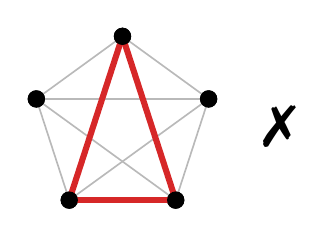
\begin{tikzpicture}[baseline=(current bounding box.north)]\draw[gray!55, line width=0.6pt] (0.000,1.150) -- (-1.094,0.355);
\draw[gray!55, line width=0.6pt] (0.000,1.150) -- (-0.676,-0.930);
\draw[gray!55, line width=0.6pt] (0.000,1.150) -- (0.676,-0.930);
\draw[gray!55, line width=0.6pt] (0.000,1.150) -- (1.094,0.355);
\draw[gray!55, line width=0.6pt] (-1.094,0.355) -- (-0.676,-0.930);
\draw[gray!55, line width=0.6pt] (-1.094,0.355) -- (0.676,-0.930);
\draw[gray!55, line width=0.6pt] (-1.094,0.355) -- (1.094,0.355);
\draw[gray!55, line width=0.6pt] (-0.676,-0.930) -- (0.676,-0.930);
\draw[gray!55, line width=0.6pt] (-0.676,-0.930) -- (1.094,0.355);
\draw[gray!55, line width=0.6pt] (0.676,-0.930) -- (1.094,0.355);
\fill (0.000,1.150) circle (0.11);
\fill (-1.094,0.355) circle (0.11);
\fill (-0.676,-0.930) circle (0.11);
\fill (0.676,-0.930) circle (0.11);
\fill (1.094,0.355) circle (0.11);
\draw[cred, line width=2.2pt] (0.000,1.150) -- (-0.676,-0.930);
\draw[cred, line width=2.2pt] (0.000,1.150) -- (0.676,-0.930);
\draw[cred, line width=2.2pt] (-0.676,-0.930) -- (0.676,-0.930);
\fill (0.000,1.150) circle (0.11);
\fill (-1.094,0.355) circle (0.11);
\fill (-0.676,-0.930) circle (0.11);
\fill (0.676,-0.930) circle (0.11);
\fill (1.094,0.355) circle (0.11);
\node[font=\huge] at (2.000,0) {\ding{55}};\end{tikzpicture}\end{minipage}\par

\vspace{4pt}\begin{center}
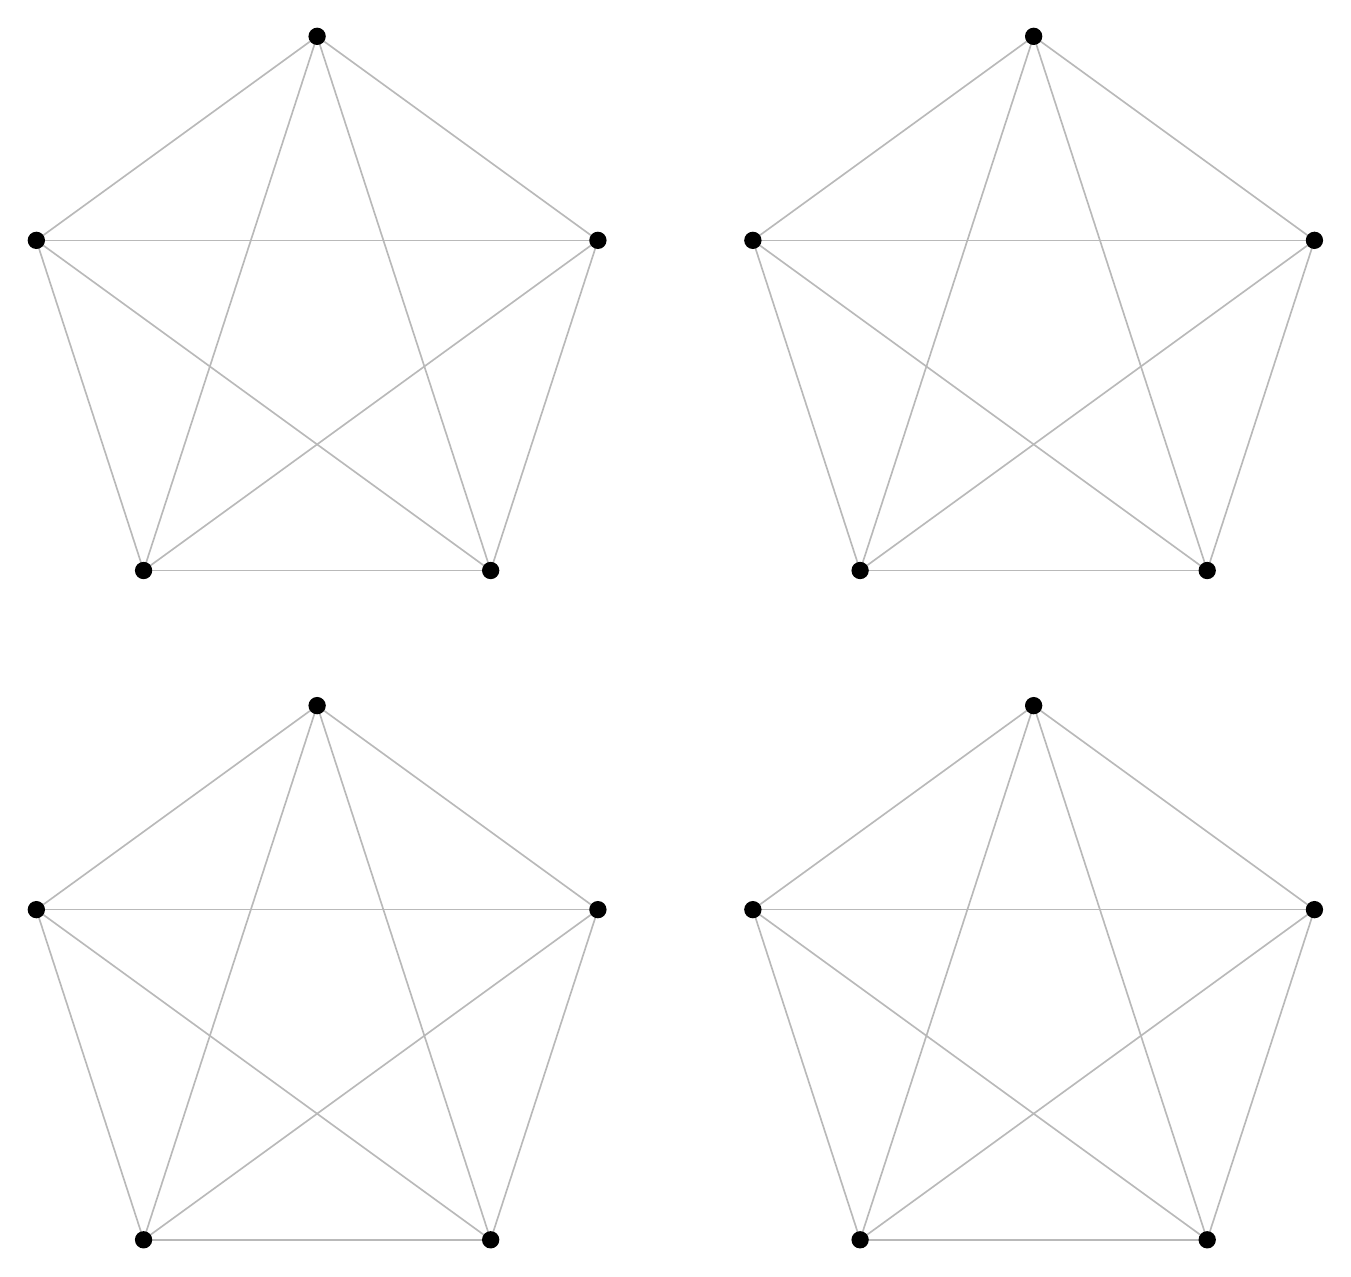
\begin{tikzpicture}
\draw[gray!55, line width=0.6pt] (0.000,3.750) -- (-3.566,1.159);
\draw[gray!55, line width=0.6pt] (0.000,3.750) -- (-2.204,-3.034);
\draw[gray!55, line width=0.6pt] (0.000,3.750) -- (2.204,-3.034);
\draw[gray!55, line width=0.6pt] (0.000,3.750) -- (3.566,1.159);
\draw[gray!55, line width=0.6pt] (-3.566,1.159) -- (-2.204,-3.034);
\draw[gray!55, line width=0.6pt] (-3.566,1.159) -- (2.204,-3.034);
\draw[gray!55, line width=0.6pt] (-3.566,1.159) -- (3.566,1.159);
\draw[gray!55, line width=0.6pt] (-2.204,-3.034) -- (2.204,-3.034);
\draw[gray!55, line width=0.6pt] (-2.204,-3.034) -- (3.566,1.159);
\draw[gray!55, line width=0.6pt] (2.204,-3.034) -- (3.566,1.159);
\fill (0.000,3.750) circle (0.11);
\fill (-3.566,1.159) circle (0.11);
\fill (-2.204,-3.034) circle (0.11);
\fill (2.204,-3.034) circle (0.11);
\fill (3.566,1.159) circle (0.11);
\draw[gray!55, line width=0.6pt] (9.100,3.750) -- (5.534,1.159);
\draw[gray!55, line width=0.6pt] (9.100,3.750) -- (6.896,-3.034);
\draw[gray!55, line width=0.6pt] (9.100,3.750) -- (11.304,-3.034);
\draw[gray!55, line width=0.6pt] (9.100,3.750) -- (12.666,1.159);
\draw[gray!55, line width=0.6pt] (5.534,1.159) -- (6.896,-3.034);
\draw[gray!55, line width=0.6pt] (5.534,1.159) -- (11.304,-3.034);
\draw[gray!55, line width=0.6pt] (5.534,1.159) -- (12.666,1.159);
\draw[gray!55, line width=0.6pt] (6.896,-3.034) -- (11.304,-3.034);
\draw[gray!55, line width=0.6pt] (6.896,-3.034) -- (12.666,1.159);
\draw[gray!55, line width=0.6pt] (11.304,-3.034) -- (12.666,1.159);
\fill (9.100,3.750) circle (0.11);
\fill (5.534,1.159) circle (0.11);
\fill (6.896,-3.034) circle (0.11);
\fill (11.304,-3.034) circle (0.11);
\fill (12.666,1.159) circle (0.11);
\draw[gray!55, line width=0.6pt] (0.000,-4.750) -- (-3.566,-7.341);
\draw[gray!55, line width=0.6pt] (0.000,-4.750) -- (-2.204,-11.534);
\draw[gray!55, line width=0.6pt] (0.000,-4.750) -- (2.204,-11.534);
\draw[gray!55, line width=0.6pt] (0.000,-4.750) -- (3.566,-7.341);
\draw[gray!55, line width=0.6pt] (-3.566,-7.341) -- (-2.204,-11.534);
\draw[gray!55, line width=0.6pt] (-3.566,-7.341) -- (2.204,-11.534);
\draw[gray!55, line width=0.6pt] (-3.566,-7.341) -- (3.566,-7.341);
\draw[gray!55, line width=0.6pt] (-2.204,-11.534) -- (2.204,-11.534);
\draw[gray!55, line width=0.6pt] (-2.204,-11.534) -- (3.566,-7.341);
\draw[gray!55, line width=0.6pt] (2.204,-11.534) -- (3.566,-7.341);
\fill (0.000,-4.750) circle (0.11);
\fill (-3.566,-7.341) circle (0.11);
\fill (-2.204,-11.534) circle (0.11);
\fill (2.204,-11.534) circle (0.11);
\fill (3.566,-7.341) circle (0.11);
\draw[gray!55, line width=0.6pt] (9.100,-4.750) -- (5.534,-7.341);
\draw[gray!55, line width=0.6pt] (9.100,-4.750) -- (6.896,-11.534);
\draw[gray!55, line width=0.6pt] (9.100,-4.750) -- (11.304,-11.534);
\draw[gray!55, line width=0.6pt] (9.100,-4.750) -- (12.666,-7.341);
\draw[gray!55, line width=0.6pt] (5.534,-7.341) -- (6.896,-11.534);
\draw[gray!55, line width=0.6pt] (5.534,-7.341) -- (11.304,-11.534);
\draw[gray!55, line width=0.6pt] (5.534,-7.341) -- (12.666,-7.341);
\draw[gray!55, line width=0.6pt] (6.896,-11.534) -- (11.304,-11.534);
\draw[gray!55, line width=0.6pt] (6.896,-11.534) -- (12.666,-7.341);
\draw[gray!55, line width=0.6pt] (11.304,-11.534) -- (12.666,-7.341);
\fill (9.100,-4.750) circle (0.11);
\fill (5.534,-7.341) circle (0.11);
\fill (6.896,-11.534) circle (0.11);
\fill (11.304,-11.534) circle (0.11);
\fill (12.666,-7.341) circle (0.11);
\end{tikzpicture}
\end{center}
\newpage
\par\noindent\textbf{Problem 7:} Play Sim with a partner on a board of six dots. One player colors lines red and the other blue. Take turns, coloring one line each turn. If you join three dots with three lines of your own color, you lose. Can a game end with all fifteen lines colored and nobody losing?\par

\vspace{4pt}\begin{center}
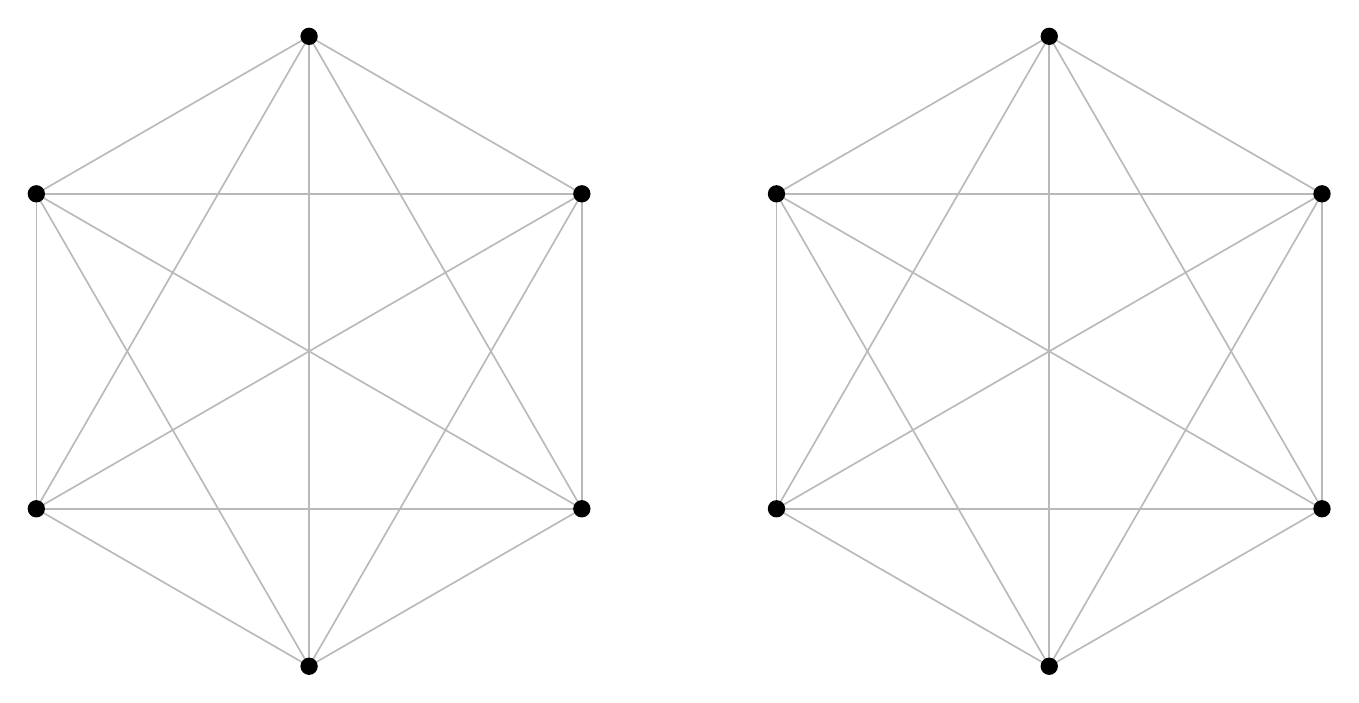
\begin{tikzpicture}
\draw[gray!55, line width=0.6pt] (0.000,4.000) -- (-3.464,2.000);
\draw[gray!55, line width=0.6pt] (0.000,4.000) -- (-3.464,-2.000);
\draw[gray!55, line width=0.6pt] (0.000,4.000) -- (-0.000,-4.000);
\draw[gray!55, line width=0.6pt] (0.000,4.000) -- (3.464,-2.000);
\draw[gray!55, line width=0.6pt] (0.000,4.000) -- (3.464,2.000);
\draw[gray!55, line width=0.6pt] (-3.464,2.000) -- (-3.464,-2.000);
\draw[gray!55, line width=0.6pt] (-3.464,2.000) -- (-0.000,-4.000);
\draw[gray!55, line width=0.6pt] (-3.464,2.000) -- (3.464,-2.000);
\draw[gray!55, line width=0.6pt] (-3.464,2.000) -- (3.464,2.000);
\draw[gray!55, line width=0.6pt] (-3.464,-2.000) -- (-0.000,-4.000);
\draw[gray!55, line width=0.6pt] (-3.464,-2.000) -- (3.464,-2.000);
\draw[gray!55, line width=0.6pt] (-3.464,-2.000) -- (3.464,2.000);
\draw[gray!55, line width=0.6pt] (-0.000,-4.000) -- (3.464,-2.000);
\draw[gray!55, line width=0.6pt] (-0.000,-4.000) -- (3.464,2.000);
\draw[gray!55, line width=0.6pt] (3.464,-2.000) -- (3.464,2.000);
\fill (0.000,4.000) circle (0.11);
\fill (-3.464,2.000) circle (0.11);
\fill (-3.464,-2.000) circle (0.11);
\fill (-0.000,-4.000) circle (0.11);
\fill (3.464,-2.000) circle (0.11);
\fill (3.464,2.000) circle (0.11);
\draw[gray!55, line width=0.6pt] (9.400,4.000) -- (5.936,2.000);
\draw[gray!55, line width=0.6pt] (9.400,4.000) -- (5.936,-2.000);
\draw[gray!55, line width=0.6pt] (9.400,4.000) -- (9.400,-4.000);
\draw[gray!55, line width=0.6pt] (9.400,4.000) -- (12.864,-2.000);
\draw[gray!55, line width=0.6pt] (9.400,4.000) -- (12.864,2.000);
\draw[gray!55, line width=0.6pt] (5.936,2.000) -- (5.936,-2.000);
\draw[gray!55, line width=0.6pt] (5.936,2.000) -- (9.400,-4.000);
\draw[gray!55, line width=0.6pt] (5.936,2.000) -- (12.864,-2.000);
\draw[gray!55, line width=0.6pt] (5.936,2.000) -- (12.864,2.000);
\draw[gray!55, line width=0.6pt] (5.936,-2.000) -- (9.400,-4.000);
\draw[gray!55, line width=0.6pt] (5.936,-2.000) -- (12.864,-2.000);
\draw[gray!55, line width=0.6pt] (5.936,-2.000) -- (12.864,2.000);
\draw[gray!55, line width=0.6pt] (9.400,-4.000) -- (12.864,-2.000);
\draw[gray!55, line width=0.6pt] (9.400,-4.000) -- (12.864,2.000);
\draw[gray!55, line width=0.6pt] (12.864,-2.000) -- (12.864,2.000);
\fill (9.400,4.000) circle (0.11);
\fill (5.936,2.000) circle (0.11);
\fill (5.936,-2.000) circle (0.11);
\fill (9.400,-4.000) circle (0.11);
\fill (12.864,-2.000) circle (0.11);
\fill (12.864,2.000) circle (0.11);
\end{tikzpicture}
\end{center}
\vspace{0.8cm}
\par\noindent\textbf{Problem 8:} Color the numbers 1, 2, 3, 4, \dots{} red, blue or green, using the rule from Problem 4. How far can you go?\par

\vspace{6pt}\begin{center}
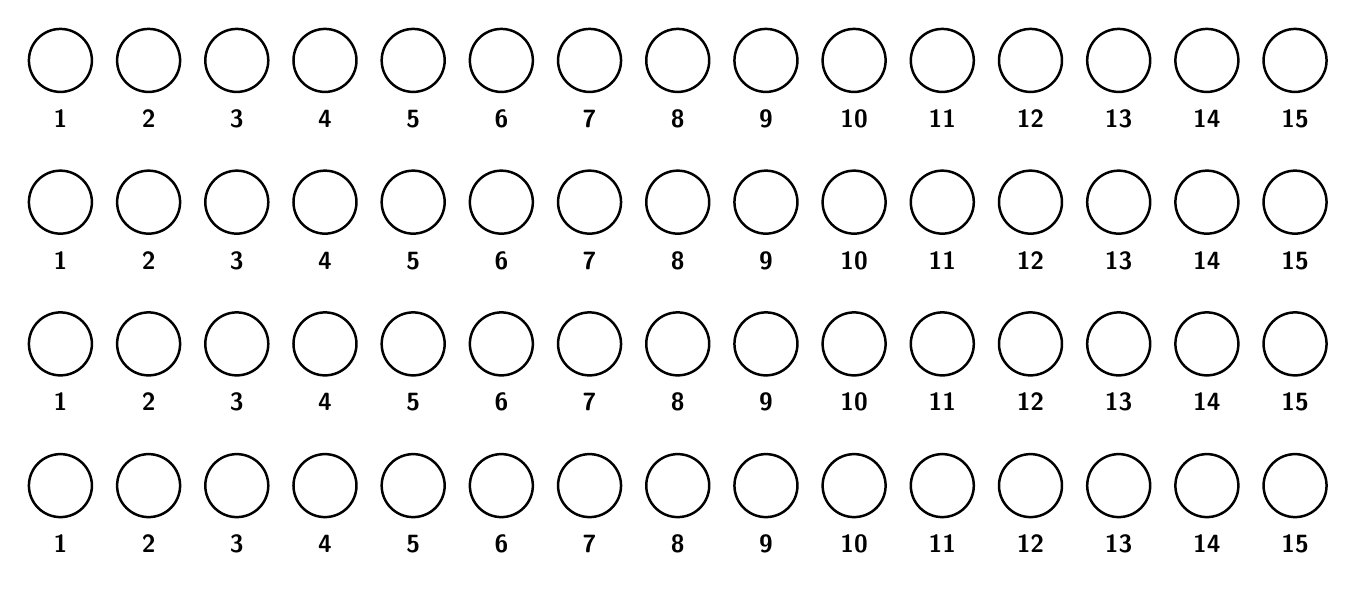
\begin{tikzpicture}
\draw[line width=0.9pt] (0.400,0.400) circle (0.400);
\node[font=\small\bfseries, anchor=base] at (0.400,-0.450) {1};
\draw[line width=0.9pt] (1.520,0.400) circle (0.400);
\node[font=\small\bfseries, anchor=base] at (1.520,-0.450) {2};
\draw[line width=0.9pt] (2.640,0.400) circle (0.400);
\node[font=\small\bfseries, anchor=base] at (2.640,-0.450) {3};
\draw[line width=0.9pt] (3.760,0.400) circle (0.400);
\node[font=\small\bfseries, anchor=base] at (3.760,-0.450) {4};
\draw[line width=0.9pt] (4.880,0.400) circle (0.400);
\node[font=\small\bfseries, anchor=base] at (4.880,-0.450) {5};
\draw[line width=0.9pt] (6.000,0.400) circle (0.400);
\node[font=\small\bfseries, anchor=base] at (6.000,-0.450) {6};
\draw[line width=0.9pt] (7.120,0.400) circle (0.400);
\node[font=\small\bfseries, anchor=base] at (7.120,-0.450) {7};
\draw[line width=0.9pt] (8.240,0.400) circle (0.400);
\node[font=\small\bfseries, anchor=base] at (8.240,-0.450) {8};
\draw[line width=0.9pt] (9.360,0.400) circle (0.400);
\node[font=\small\bfseries, anchor=base] at (9.360,-0.450) {9};
\draw[line width=0.9pt] (10.480,0.400) circle (0.400);
\node[font=\small\bfseries, anchor=base] at (10.480,-0.450) {10};
\draw[line width=0.9pt] (11.600,0.400) circle (0.400);
\node[font=\small\bfseries, anchor=base] at (11.600,-0.450) {11};
\draw[line width=0.9pt] (12.720,0.400) circle (0.400);
\node[font=\small\bfseries, anchor=base] at (12.720,-0.450) {12};
\draw[line width=0.9pt] (13.840,0.400) circle (0.400);
\node[font=\small\bfseries, anchor=base] at (13.840,-0.450) {13};
\draw[line width=0.9pt] (14.960,0.400) circle (0.400);
\node[font=\small\bfseries, anchor=base] at (14.960,-0.450) {14};
\draw[line width=0.9pt] (16.080,0.400) circle (0.400);
\node[font=\small\bfseries, anchor=base] at (16.080,-0.450) {15};
\draw[line width=0.9pt] (0.400,-1.400) circle (0.400);
\node[font=\small\bfseries, anchor=base] at (0.400,-2.250) {1};
\draw[line width=0.9pt] (1.520,-1.400) circle (0.400);
\node[font=\small\bfseries, anchor=base] at (1.520,-2.250) {2};
\draw[line width=0.9pt] (2.640,-1.400) circle (0.400);
\node[font=\small\bfseries, anchor=base] at (2.640,-2.250) {3};
\draw[line width=0.9pt] (3.760,-1.400) circle (0.400);
\node[font=\small\bfseries, anchor=base] at (3.760,-2.250) {4};
\draw[line width=0.9pt] (4.880,-1.400) circle (0.400);
\node[font=\small\bfseries, anchor=base] at (4.880,-2.250) {5};
\draw[line width=0.9pt] (6.000,-1.400) circle (0.400);
\node[font=\small\bfseries, anchor=base] at (6.000,-2.250) {6};
\draw[line width=0.9pt] (7.120,-1.400) circle (0.400);
\node[font=\small\bfseries, anchor=base] at (7.120,-2.250) {7};
\draw[line width=0.9pt] (8.240,-1.400) circle (0.400);
\node[font=\small\bfseries, anchor=base] at (8.240,-2.250) {8};
\draw[line width=0.9pt] (9.360,-1.400) circle (0.400);
\node[font=\small\bfseries, anchor=base] at (9.360,-2.250) {9};
\draw[line width=0.9pt] (10.480,-1.400) circle (0.400);
\node[font=\small\bfseries, anchor=base] at (10.480,-2.250) {10};
\draw[line width=0.9pt] (11.600,-1.400) circle (0.400);
\node[font=\small\bfseries, anchor=base] at (11.600,-2.250) {11};
\draw[line width=0.9pt] (12.720,-1.400) circle (0.400);
\node[font=\small\bfseries, anchor=base] at (12.720,-2.250) {12};
\draw[line width=0.9pt] (13.840,-1.400) circle (0.400);
\node[font=\small\bfseries, anchor=base] at (13.840,-2.250) {13};
\draw[line width=0.9pt] (14.960,-1.400) circle (0.400);
\node[font=\small\bfseries, anchor=base] at (14.960,-2.250) {14};
\draw[line width=0.9pt] (16.080,-1.400) circle (0.400);
\node[font=\small\bfseries, anchor=base] at (16.080,-2.250) {15};
\draw[line width=0.9pt] (0.400,-3.200) circle (0.400);
\node[font=\small\bfseries, anchor=base] at (0.400,-4.050) {1};
\draw[line width=0.9pt] (1.520,-3.200) circle (0.400);
\node[font=\small\bfseries, anchor=base] at (1.520,-4.050) {2};
\draw[line width=0.9pt] (2.640,-3.200) circle (0.400);
\node[font=\small\bfseries, anchor=base] at (2.640,-4.050) {3};
\draw[line width=0.9pt] (3.760,-3.200) circle (0.400);
\node[font=\small\bfseries, anchor=base] at (3.760,-4.050) {4};
\draw[line width=0.9pt] (4.880,-3.200) circle (0.400);
\node[font=\small\bfseries, anchor=base] at (4.880,-4.050) {5};
\draw[line width=0.9pt] (6.000,-3.200) circle (0.400);
\node[font=\small\bfseries, anchor=base] at (6.000,-4.050) {6};
\draw[line width=0.9pt] (7.120,-3.200) circle (0.400);
\node[font=\small\bfseries, anchor=base] at (7.120,-4.050) {7};
\draw[line width=0.9pt] (8.240,-3.200) circle (0.400);
\node[font=\small\bfseries, anchor=base] at (8.240,-4.050) {8};
\draw[line width=0.9pt] (9.360,-3.200) circle (0.400);
\node[font=\small\bfseries, anchor=base] at (9.360,-4.050) {9};
\draw[line width=0.9pt] (10.480,-3.200) circle (0.400);
\node[font=\small\bfseries, anchor=base] at (10.480,-4.050) {10};
\draw[line width=0.9pt] (11.600,-3.200) circle (0.400);
\node[font=\small\bfseries, anchor=base] at (11.600,-4.050) {11};
\draw[line width=0.9pt] (12.720,-3.200) circle (0.400);
\node[font=\small\bfseries, anchor=base] at (12.720,-4.050) {12};
\draw[line width=0.9pt] (13.840,-3.200) circle (0.400);
\node[font=\small\bfseries, anchor=base] at (13.840,-4.050) {13};
\draw[line width=0.9pt] (14.960,-3.200) circle (0.400);
\node[font=\small\bfseries, anchor=base] at (14.960,-4.050) {14};
\draw[line width=0.9pt] (16.080,-3.200) circle (0.400);
\node[font=\small\bfseries, anchor=base] at (16.080,-4.050) {15};
\draw[line width=0.9pt] (0.400,-5.000) circle (0.400);
\node[font=\small\bfseries, anchor=base] at (0.400,-5.850) {1};
\draw[line width=0.9pt] (1.520,-5.000) circle (0.400);
\node[font=\small\bfseries, anchor=base] at (1.520,-5.850) {2};
\draw[line width=0.9pt] (2.640,-5.000) circle (0.400);
\node[font=\small\bfseries, anchor=base] at (2.640,-5.850) {3};
\draw[line width=0.9pt] (3.760,-5.000) circle (0.400);
\node[font=\small\bfseries, anchor=base] at (3.760,-5.850) {4};
\draw[line width=0.9pt] (4.880,-5.000) circle (0.400);
\node[font=\small\bfseries, anchor=base] at (4.880,-5.850) {5};
\draw[line width=0.9pt] (6.000,-5.000) circle (0.400);
\node[font=\small\bfseries, anchor=base] at (6.000,-5.850) {6};
\draw[line width=0.9pt] (7.120,-5.000) circle (0.400);
\node[font=\small\bfseries, anchor=base] at (7.120,-5.850) {7};
\draw[line width=0.9pt] (8.240,-5.000) circle (0.400);
\node[font=\small\bfseries, anchor=base] at (8.240,-5.850) {8};
\draw[line width=0.9pt] (9.360,-5.000) circle (0.400);
\node[font=\small\bfseries, anchor=base] at (9.360,-5.850) {9};
\draw[line width=0.9pt] (10.480,-5.000) circle (0.400);
\node[font=\small\bfseries, anchor=base] at (10.480,-5.850) {10};
\draw[line width=0.9pt] (11.600,-5.000) circle (0.400);
\node[font=\small\bfseries, anchor=base] at (11.600,-5.850) {11};
\draw[line width=0.9pt] (12.720,-5.000) circle (0.400);
\node[font=\small\bfseries, anchor=base] at (12.720,-5.850) {12};
\draw[line width=0.9pt] (13.840,-5.000) circle (0.400);
\node[font=\small\bfseries, anchor=base] at (13.840,-5.850) {13};
\draw[line width=0.9pt] (14.960,-5.000) circle (0.400);
\node[font=\small\bfseries, anchor=base] at (14.960,-5.850) {14};
\draw[line width=0.9pt] (16.080,-5.000) circle (0.400);
\node[font=\small\bfseries, anchor=base] at (16.080,-5.850) {15};
\end{tikzpicture}
\end{center}
\end{document}
